% !TeX program = xelatex
\RequirePackage{fix-cm}
\documentclass[14pt,a4paper]{extarticle}
\usepackage{fontspec}
\defaultfontfeatures{Ligatures=TeX}
\input{build/font-path.tex}
\ifdefined\reportFontPath
  \setmainfont{Times.TTF}[Path=\reportFontPath,BoldFont=Timesbd.TTF,ItalicFont=Timesi.TTF,BoldItalicFont=Timesbi.TTF]
  \newfontfamily\cyrillicfont{Times.TTF}[Path=\reportFontPath,BoldFont=Timesbd.TTF,ItalicFont=Timesi.TTF,BoldItalicFont=Timesbi.TTF,Script=Default]
\else
  \setmainfont{Times New Roman}
  \newfontfamily\cyrillicfont{Times New Roman}
\fi
\setmonofont{FreeMono}
\newfontfamily\cyrillicfonttt{FreeMono}
\usepackage{polyglossia}
\setdefaultlanguage{russian}
\setotherlanguage{english}
\usepackage[left=30mm,right=10mm,top=20mm,bottom=20mm,footskip=10mm]{geometry}
\usepackage{setspace}
\makeatletter
\renewcommand{\normalsize}{\@setfontsize\normalsize{14bp}{16.8bp}}
\makeatother
\onehalfspacing
\AtBeginDocument{\normalsize}
\setlength{\parindent}{1.25cm}
\setlength{\parskip}{0pt}
\usepackage{indentfirst}
\usepackage{array,tabularx,graphicx,float,caption,fvextra,xcolor}
\DeclareCaptionLabelSeparator{gost}{~—~}
\captionsetup{font=small,labelsep=gost,justification=centering,singlelinecheck=false}
\captionsetup[table]{justification=raggedright,position=top,skip=6pt}
\captionsetup[figure]{skip=8pt}
\addto\captionsrussian{\renewcommand{\figurename}{Рисунок}\renewcommand{\tablename}{Таблица}}
\usepackage{titlesec}
\titleformat{\section}[block]{\normalfont\bfseries\centering}{\thesection.}{.5em}{\MakeUppercase}
\titlespacing*{\section}{0pt}{0pt}{18pt}
\usepackage{enumitem}
\usepackage{xurl}
\urlstyle{same}
\usepackage[hidelinks,unicode,pdfauthor={Матвеев М. А.},pdftitle={Лабораторная работа №2. Работа с таблицами}]{hyperref}
\pagestyle{plain}
\emergencystretch=2em
\clubpenalty=10000
\widowpenalty=10000
\raggedbottom
\newcolumntype{Y}{>{\raggedright\arraybackslash}X}
\newcommand{\code}[1]{{\fontsize{12}{14}\selectfont\texttt{#1}}}
\input{build/highlight-style.tex}
\newcommand{\listing}[1]{\begingroup\singlespacing\setlength{\topsep}{0pt}\setlength{\partopsep}{0pt}\input{build/#1.tex}\endgroup}

\begin{document}
\begin{titlepage}
\thispagestyle{empty}
\begin{center}
\bfseries
МИНОБРНАУКИ РОССИИ\\
Федеральное государственное автономное\\
образовательное учреждение высшего образования\\
«Санкт-Петербургский государственный\\
электротехнический университет «ЛЭТИ»\\
им. В.И. Ульянова (Ленина)»\\
Кафедра информационных систем
\end{center}
\vspace{30mm}
\begin{center}
\textbf{ОТЧЕТ ПО ЛАБОРАТОРНОЙ РАБОТЕ №2}\\[8mm]
«Работа с таблицами»
\end{center}
\vfill
\noindent\begin{tabularx}{\textwidth}{@{}lXr@{}}
Студент гр. 4372 & \centering\rule{25mm}{0.3pt} & Матвеев М. А.\\[8mm]
Преподаватель & \centering\rule{25mm}{0.3pt} & Нечитайленко Р. А.\\
\end{tabularx}
\vspace{20mm}
\begin{center}
Санкт-Петербург\\
2026
\end{center}
\end{titlepage}
\setcounter{page}{2}

\section{Цель и выполнение работы}
Цель работы: создать и оформить таблицу с заголовком, данными и итоговой строкой.

Таблица содержит пять строк и пять столбцов. Заголовок размещён в \code{thead}, три строки данных в \code{tbody}, итог в \code{tfoot}. Атрибут \code{colspan="5"} объединяет ячейки итоговой строки с текстом «Всего: 3».

Ширина таблицы составляет 500~px. Свойство \code{border-collapse} со значением \code{collapse} объединяет соседние границы. Для ячеек заданы сплошная граница толщиной 1~px цвета \code{\#ccc}, вертикальные отступы 5~px и горизонтальные отступы 10~px.

Фон заголовка имеет цвет \code{\#f0f1f4}. В итоговой строке белый текст выровнен по правому краю на фоне \code{\#121212}.
\begin{figure}[H]
\centering
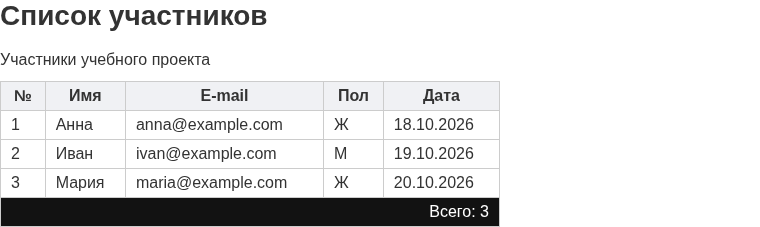
\includegraphics[width=\textwidth,height=100mm,keepaspectratio]{assets/desktop.png}
\caption{Таблица участников}
\end{figure}

\vspace{6mm}
\section{Проверка и результат}
Проверка в Chromium 153 подтвердила структуру таблицы, объединение ячеек итоговой строки и заданные стили.

При ширине окна 320 и 375~px таблица сохраняет ширину 500~px и прокручивается внутри контейнера. Страница при этом не выходит за пределы окна. Контейнер доступен с клавиатуры.


\clearpage
\section{Исходный код: index.html}
\listing{index.html}

\clearpage
\section{Исходный код: style.scss}
\listing{style.scss}
\clearpage
\section*{Список использованных источников}
\begin{enumerate}[label=\arabic*.,leftmargin=8mm,itemsep=8pt,parsep=0pt]
\item Тег <table> // HTMLbook.ru. URL: \url{https://htmlbook.ru/html/table}.
\item Тег <thead> // HTMLbook.ru. URL: \url{https://htmlbook.ru/html/thead}.
\item Атрибут colspan // HTMLbook.ru. URL: \url{https://htmlbook.ru/html/td/colspan}.
\item border-collapse // HTMLbook.ru. URL: \url{https://htmlbook.ru/css/border-collapse}.
\item Dart Sass Command-Line Interface // Sass. URL: \url{https://sass-lang.com/documentation/cli/dart-sass/}.
\end{enumerate}
\end{document}
